\begin{comment}
- Gibs phenomenon
- Post-processing used (how impactful is removing non-distinct solutions?)
- How does clean TVD evolve with JVV steps (see proof)?
- Approximation ratio
- Numerical analysis (which mean to take)
\end{comment}

\chapter{Résolution de problèmes \textsf{\#P}-complet avec VQCount}

%-----------------------------------------------------------------------------%

\begin{comment}
\subsection*{Plan}

\begin{enumerate}
    \item Mentionner les problèmes étudiés
    \item Mentionner les méthodes utilisées (réseaux de tenseurs)
    \item Décrire les paramètres de l'étude (nombre d'instances, régimes de complexité, etc.)
    \item Expliquer les principaux résultats (compromis entre QAOA et GM-QAOA)
\end{enumerate}

\subsection*{Références}
\end{comment}

Dans la section précédente, un cadre théorique s'appuyant sur l'algorithme de JVV a été construit pour la résolution de problèmes de comptage à l'aide d'algorithmes variationnels quantiques. L'algorithme résultant, VQCount, obtient un compte approximatif à une erreur multiplicative près en échantillonnant un nombre polynomial de solutions à un circuit quantique optimisé GM-QAOA. Toutefois, plusieurs conditions potentiellement dispensables ou difficilement applicables ont été imposées. Cette section change l'optique précédente en évaluant l'algorithme VQCount uniquement en tant que méthode heuristique, c'est-à-dire en caractérisant l'algorithme sans se soucier des garanties. La résolution de deux problèmes \textsf{\#P}-complet, \#NAE3SAT et \#1in3SAT, sont étudiés.

%-----------------------------------------------------------------------------%

\section{Paramètres de l'étude}


Certaines précédentes considérations sont ainsi relâchées ou modifiées. D'abord, l'algorithme GM-QAOA n'est plus considéré dans sa forme limite de Grover. Les paramètres $(\vec{\alpha}, \vec{\beta})$ sont optimisées plutôt que d'utiliser des paramètres fixes. De plus, les problèmes étudiés sont transformé à des Hamiltoniens de problème régulier contenant une tour d'états excités plutôt que de l'oracle à deux niveaux construits précédemment.

L'algorithme VQCount est appliqué aux problèmes \#NAE3SAT positif et \#1-in-3SAT positif présentés à la section~\ref{sec:satisfaisabilite-booleenne}. Le problème \#NAE3SAT est difficile près du seuil de satisfaisabilité situé au ratio de clauses sur variables critique $\alpha_{c} \approx 2.1$. Pour étudier l'effet de la complexité des formules aléatoires sur la performance de VQCount, des instances sont générées à $\alpha = 1$ et $\alpha = 2$. Celles-ci sont générées à partir de graphes connectés bipartis, imposant une restriction supplémentaire. Similairement, les instances du problème \#1-in-3SAT positive sont à leur seuil de difficulté le plus élevé près de $\alpha_{c} \approx 2/3$. Pour étudier ce problème dans le régime difficile, les instances sont générées à partir de graphes aléatoires cubiques, en plaçant une clause sur tous les sommets et une variable sur toutes les arrêtes. Ce type de problème appartient à la catégorie des problèmes verrouillés, décrit à la section~\ref{sec:transitions-de-phase}, étant vraisemblablement les plus difficiles des problèmes \#P. Par la suite, les instances générées sont convertis en un modèle d'Ising à l'aide de la transformation décrite à la section~\ref{subsec:encodage-probleme}.

La simulation de circuits quantiques est un problème complexe en raison de la quantité de mémoire nécessaire pour représenter l'espace d'Hilbert. La méthode la plus utilisée, la simulation à vecteur d'état, ne peut atteindre plus d'une vingtaine de qubits pour cette raison. Les réseaux de tenseur sont un outil alternatif puissant, particulièrement pour l'étude de circuits quantiques peu profonds. L'annexe~\ref{cha:reseaux-de-tenseurs} introduit les réseaux de tenseur et les méthodes particulières utilisées pour la simulation de l'algorithme VQCount. La librairie « Quimb »~\cite{grayQuimbPythonPackage2018} est utilisé pour modéliser l'optimisation et l'échantillonnage des circuits quantiques QAOA et GM-QAOA. Les paramètres de ces circuits sont optimisés avec la programmation séquentielle des moindres carrés tel qu'implémenté par la librairie « SciPy »~\cite{virtanenSciPy10Fundamental2020}. Pour évaluer la validité des résultats obtenus, « Ganak »~\cite{sharmaGANAKScalableProbabilistic2019}, un compteur de modèles exact basé sur une approche probabiliste, est utilisé pour trouver le nombre exact de solutions et le solveur SAT « Glucose3 »~\cite{eenExtensibleSATsolver2004,audemardPredictingLearntClauses2009} , implémenté dans l'ensemble d'outils « PySAT »~\cite{ignatievPySATPythonToolkit2018}, est utilisé pour énumérer toutes les solutions.

Pour le problème \#NAE3SAT, 20 instances aléatoires sont générées par taille d'instance, allant de 6 à 20 variables, pour les deux densités de clause $\alpha=1$ et $\alpha = 2$. Similairement, problème \#1-in-3SAT, 20 instances aléatoires sont générées pour une taille de variable allant de 9 à 27 variables par saut de 3 variables, pour une densité de clause $\alpha = 2/3$. 

%-----------------------------------------------------------------------------%

\section{Méthode}

Afin de déterminer le nombre d'échantillons nécessaires pour atteindre un compte approximatif avec une tolérance $\varepsilon$ et une confiance $\delta$, il faut augmenter le nombre d'échantillons utilisé par l'algorithme VQCount jusqu'à ce que le nombre de solutions trouvé soit à une erreur multiplicative $\varepsilon$ du nombre de solutions exact avec une probabilité supérieure à $\delta$. La simulation de l'algorithme étant coûteuse, une méthode plus simple et moins rigoureuse est utilisée ici. L'algorithme VQCount est exécuté en augmentant le nombre de solutions échantillonnées du circuit quantique optimisé QAOA jusqu'à ce que le nombre de solutions soit à l'intérieur des bornes d'erreur $\varepsilon$. La figure~\ref{fig:count-accuracy.pdf} montre la précision du comptage, c'est-à-dire le nombre de solutions approximatif sur le nombre de solutions exact, pour différentes erreurs multiplicatives $\varepsilon$. Notons que pour diminuer les incertitudes, une procédure de lissage est utilisée. L'algorithme de JVV semble sous-estimer le nombre de solutions, comme vu avec la courbe de \#NAE3SAT avec $\alpha = 1$. Ce comportement s'explique par le manque d'échantillons indiscernables dans la distribution de probabilité des solutions échantillonnées, entraînant une légère inexactitude des probabilités dans l'arbre des configurations. 

\begin{figure}[ht!]
    \centering
    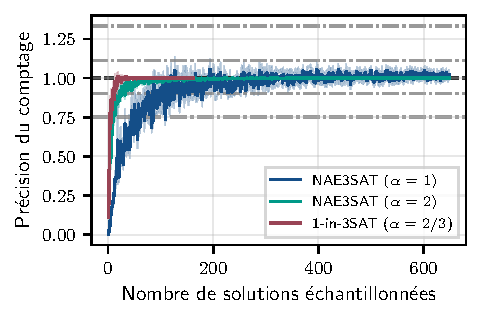
\includegraphics[width=0.5\textwidth]{figures/count-accuracy.pdf}
    \caption{}
    \label{fig:count-accuracy.pdf}
\end{figure}

%-----------------------------------------------------------------------------%

\section{Biais d'échantillonnage}

\begin{comment}
\subsection*{Plan}

\begin{enumerate}
    \item Décrire le comportement de la non-uniformité pour les différents problèmes (ne pas oublier 2SAT)
\end{enumerate}
\end{comment}

Comme vu à la section~\ref{sec:echantillonage-et-biais}, l'état préparé par un circuit GM-QAOA permet un échantillonnage uniforme de solutions tel que nécessaire pour l'algorithme de JVV, alors que la probabilité de certaines solutions est exponentiellement petite avec l'approche QAOA. Sachant que les problèmes étudiés possèdent en moyenne un nombre exponentiel de solutions et qu'un nombre polynomial d'échantillons est nécessaire, il est possible que la distribution préparée par QAOA soit suffisante pour obtenir un compte approximatif convenable. La figure~\ref{fig:nae3sat-number-of-samples} résume les résultats obtenus pour le problème \#NAE3SAT avec un circuit de profondeur $p=3$. Les figures~\ref{fig:nae3sat-number-of-samples}(a) et~\ref{fig:nae3sat-number-of-samples}(b) confirme que GM-QAOA échantillonne les solutions parfaitement uniformément. Au contraire, la distribution des solutions préparées par QAOA est de plus en plus non-uniforme avec la taille de l'instance. Les figures~\ref{fig:nae3sat-number-of-samples}(c) et~\ref{fig:nae3sat-number-of-samples}(d) montrent que, pour une profondeur de circuit fixe, le taux de succès de QAOA et GM-QAOA diminue grossièrement de façon exponentielle avec le nombre de variables, malgré que la diminution est plus importante pour GM-QAOA. Les taux de succès sont plus faibles et se détériorent plus rapidement pour $\alpha = 2$ que pour $\alpha=1$, reflétant la différence de complexité du problème selon la proximité du seuil de satisfaisabilité.

Le nombre total d'échantillons requis pour que l'algorithme VQCount retourne un compte approximatif à une erreur multiplicative $\varepsilon = 1/3$ est présenté à la figure~\ref{fig:nae3sat-number-of-samples}(e) et~\ref{fig:nae3sat-number-of-samples}(f). Le nombre d'échantillons augmente exponentiellement avec la taille des instances en raison de la post-sélection des solutions à la fois pour QAOA et GM-QAOA comme générateurs de solutions. Malgré le taux de succès exponentiellement plus faible de GM-QAOA, VQCount nécessite environ le même nombre d'échantillons avec QAOA ou GM-QAOA pour $\alpha=1$. Au contraire, VQCount avec QAOA requiert un nombre exponentiellement plus faible qu'avec GM-QAOA, malgré la non-uniformité de la distribution des probabilités de QAOA. Cela suggère que QAOA est potentiellement un générateur plus efficace pour VQCount dans le cas où les solutions soient rares et dispersées.

\begin{figure}[ht!]
    \centering
    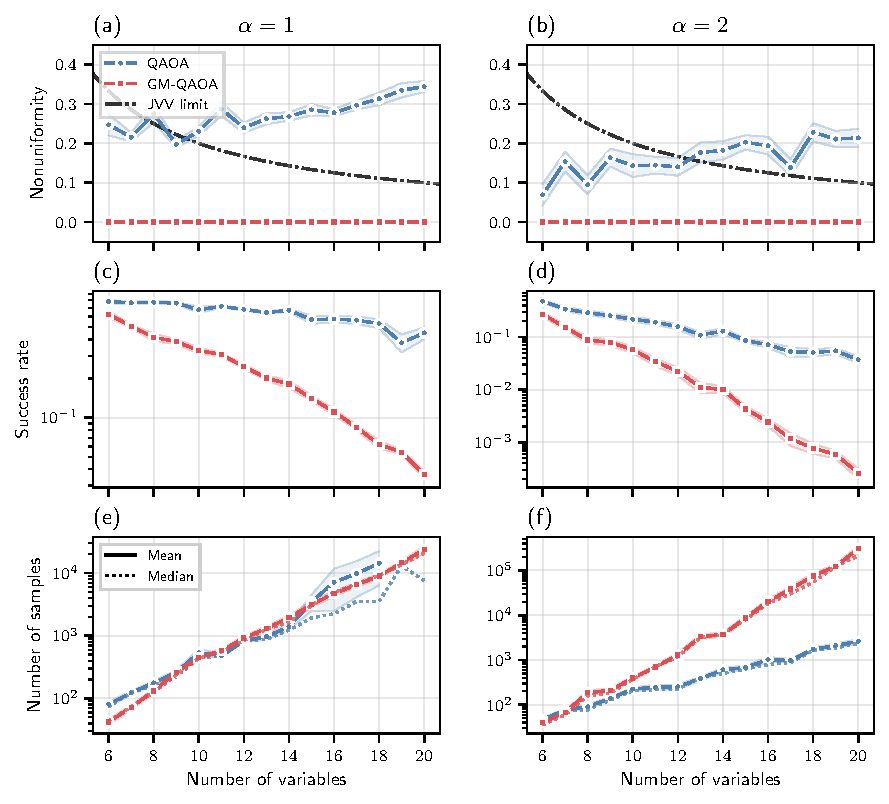
\includegraphics[width=1\textwidth]{figures/nae3sat-number-of-samples.pdf}
    \caption{}
    \label{fig:nae3sat-number-of-samples}
\end{figure}

\begin{figure}[ht!]
    \centering
    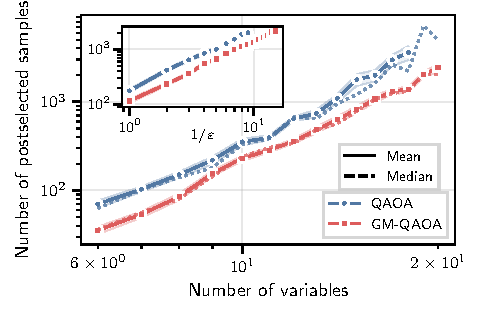
\includegraphics[width=0.5\textwidth]{figures/nae3sat-scaling.pdf}
    \caption{}
    \label{fig:nae3sat-scaling}
\end{figure}

Dans cette étude, les paramètres des circuits quantiques sont maintenus à une profondeur fixe lors de la procédure de JVV comme la ré-optimisation est coûteuse à simuler classiquement. Est-ce que ce choix a un impact important sur la performance de l'algorithme VQCount? Sachant qu'à chaque étape de l'algorithme de JVV un problème plus petit est échantillonné, il est raisonnable de s'attendre à ce que le succès de l'algorithme augmente. Comme illustré à la figure~\ref{fig:nae3sat-jvv-steps}, la non-uniformité diminue en moyenne lorsque des qubits additionnels sont fixés pour GM-QAOA. 

\textcolor{mydarkred}{\textit{Changer!}}

\begin{figure}[ht!]
    \centering
    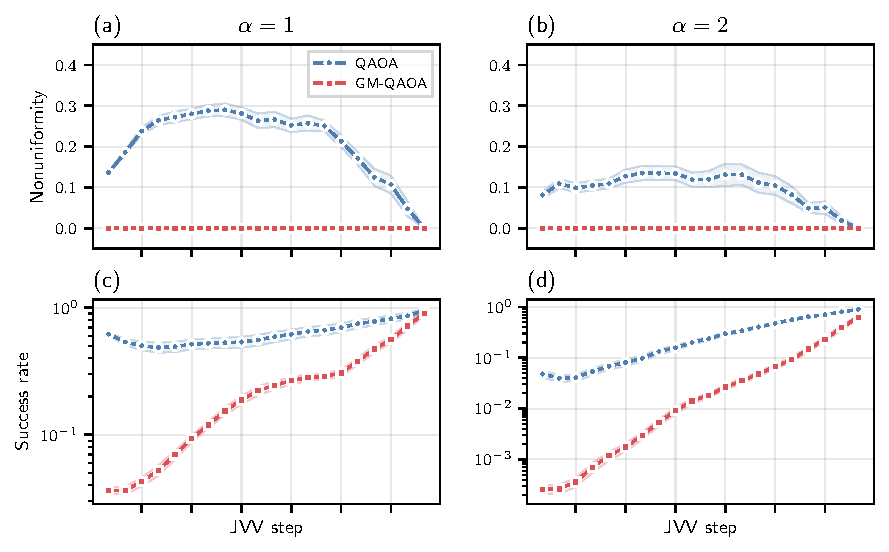
\includegraphics[width=1\textwidth]{figures/nae3sat-jvv-steps}
    \caption{}
    \label{fig:nae3sat-jvv-steps}
\end{figure}

Les résultats précédents suggèrent que le circuit QAOA est un meilleur générateur de solutions que le circuit GM-QAOA pour une faible profondeur. GM-QAOA dépend aussi d'une porte contrôle à $n$ qubits, difficilement implémentable pour la simulation classique et pour les ordinateurs quantiques bruités à court-terme. 


Pour l'instant, la performance de VQCount a été étudié pour des circuits de profondeur fixe. La figure~\ref{fig:nae3sat-depth} montre que, lorsque la profondeur du circuit augmente, la non-uniformité diminue et la probabilité d'obtenir une solution augmente, menant à un nombre d'échantillons nécessaires pour atteindre un compte approximatif avec une erreur multiplicative donnée. QAOA semble s'améliorer plus rapidement que GM-QAOA, mais la non-uniformité de QAOA augmente et atteint un plateau avec la profondeur du circuit.

\begin{figure}[ht!]
    \centering
    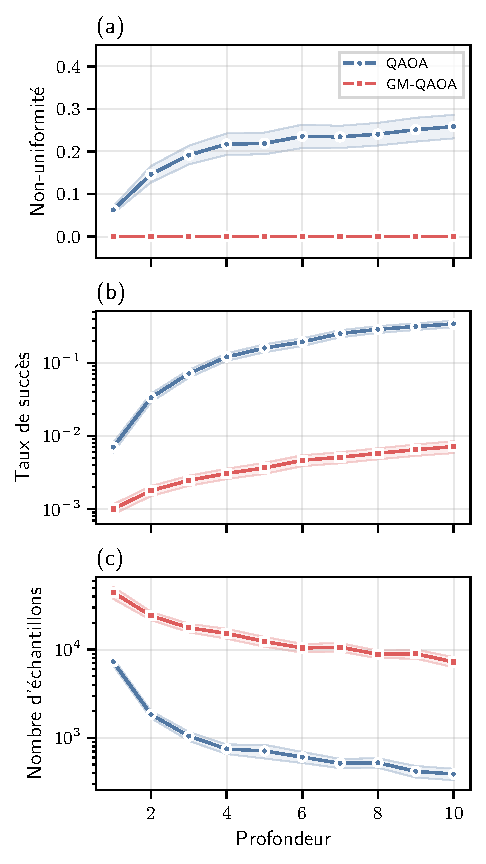
\includegraphics[width=0.5\textwidth]{figures/nae3sat-depth.pdf}
    \caption{}
    \label{fig:nae3sat-depth}
\end{figure}

%-----------------------------------------------------------------------------%

\section{Performance}

\begin{comment}
    \subsection*{Plan}
    
    \begin{enumerate}
    \item  Décrire le taux de réussite et le nombre d'échantillons requis
    \item  Décrire la performance de l'algorithme en fonction de la profondeur du circuit
    \item Décrire l'efficacité d'échantillonnage et la précision du compte
    \item Présenter brièvement le ratio d'approximation
    \end{enumerate}
\end{comment}


Ayant conclu que QAOA semble être un meilleur générateur de solutions pour une faible profondeur de circuit, la performance de VQCount avec QAOA est caractérisé de manière approfondie pour le problème \#1-in-3SAT. La figure~\ref{fig:1in3sat-number-of-samples} résume le comportement de mise à l'échelle de VQCount avec un circuit QAOA à faible profondeur. Naïvement, le nombre de solutions peut être trouvé en déterminant la probabilité qu'une chaîne de bit aléatoire échantillons de l'ensemble des chaînes de bits possible soit une solution. Comme vu à la figure~\ref{fig:1in3sat-number-of-samples}a, VQCount possède une loi d'échelle exponentiellement meilleure qu'avec un échantillonnage par rejet naïf et sa performance s'améliore avec la taille du circuit. Aux profondeurs de circuit possibles d'atteindre en utilisant des ressources computationnelles raisonnables, la performance asymptotique de VQCount est plus faible que les solveurs classiques de pointe pour ce problème~\cite{kourtisFastCountingTensor2019}, mais les résultats suggèrent que ce n'est possiblement pas le cas pour des profondeurs de circuit finies plus grandes. La précision de VQCount peut être améliorée en augmentant le nombre d'échantillons, comme montré à la figure \ref{fig:1in3sat-number-of-samples}b.

\begin{figure}[ht!]
    \centering
    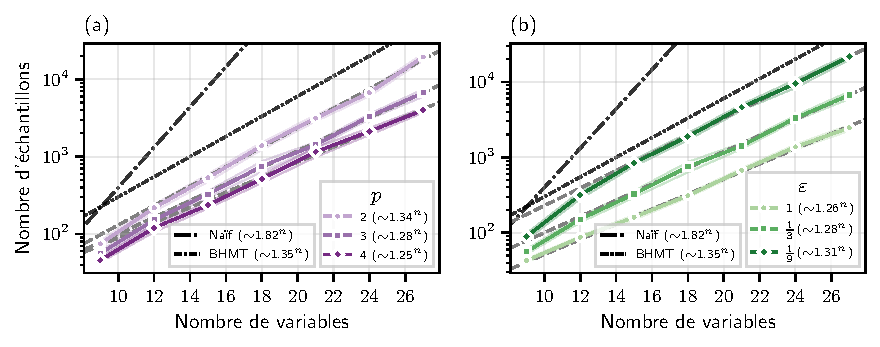
\includegraphics[width=0.5\textwidth]{figures/1in3sat-number-of-samples.pdf}
    \caption{}
    \label{fig:1in3sat-number-of-samples}
\end{figure}

\begin{figure}[ht!]
    \centering
    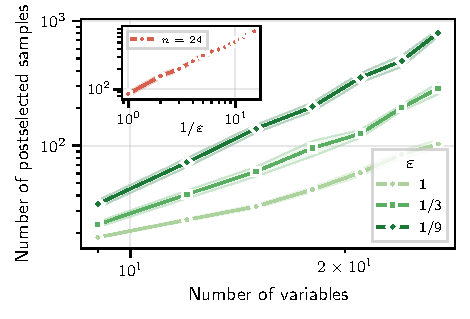
\includegraphics[width=0.5\textwidth]{figures/1in3sat-scaling.pdf}
    \caption{}
    \label{fig:1in3sat-scaling}
\end{figure}

\begin{figure}[ht!]
    \centering
    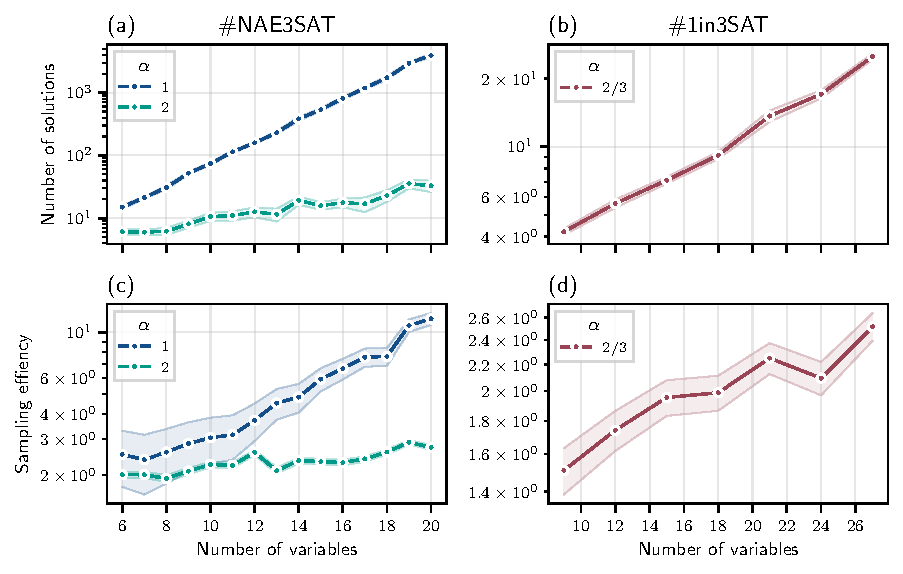
\includegraphics[width=1\textwidth]{figures/sampling-efficiency.pdf}
    \caption{}
    \label{fig:sampling-efficiency}
\end{figure}

%-----------------------------------------------------------------------------%
